%======================================================================
\chapter{Liquid-Filled HCPCF}
%======================================================================
In this chapter follows a background on different filling methods, the integrity of the scaling laws, and transmission of liquid-filled HCPCF.
\section{Experimental Set-Up}
\begin{figure}[!htb]
	\centering
	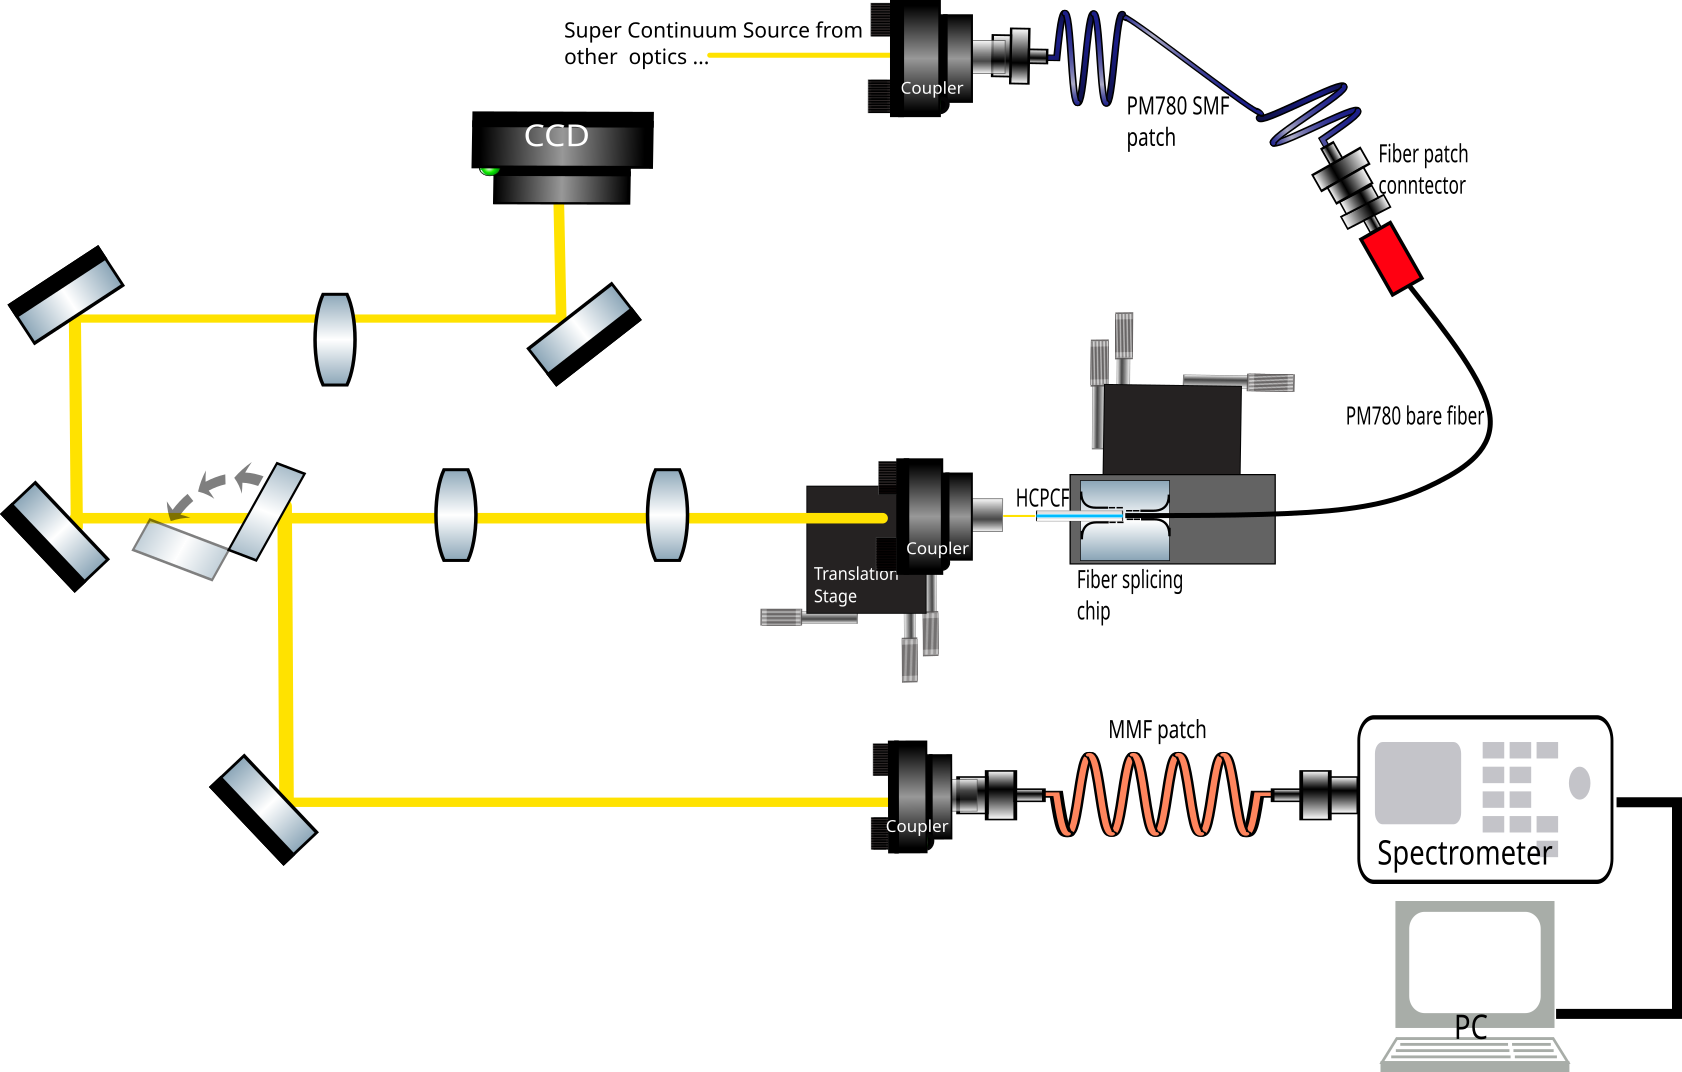
\includegraphics[width=0.75\textwidth]{./Figures/fiberfilling/Transmission_SetUp.png}
	\caption{Fiber transmission experimental set-up. The path to the CCD camera is used to monitor the modeshape coming out of the fiber and the path to the spectrometer is used to measure the transmission spectrum of the fiber.}
	\label{fig:filling exp}
\end{figure}
For the transmission measurements, shown in Fig.\ref{fig:filling exp}, fibers were cut to be between 6cm and 8cm in length. To ensure consistent coupling and positioning, light was coupled to the core of the fiber by connecting to a solid-core PM780HP fiber via a mechanical splicing chip \cite{maruf}.\\
In our experiments two different filling methods are tested: full fiber filling, and selective filling, as well as two filling liquids: deionized water (which will be referred to as DI Water or H${}_2$O) and heavy water D${}_2$O.
\begin{figure}[!htb]
	\centering
	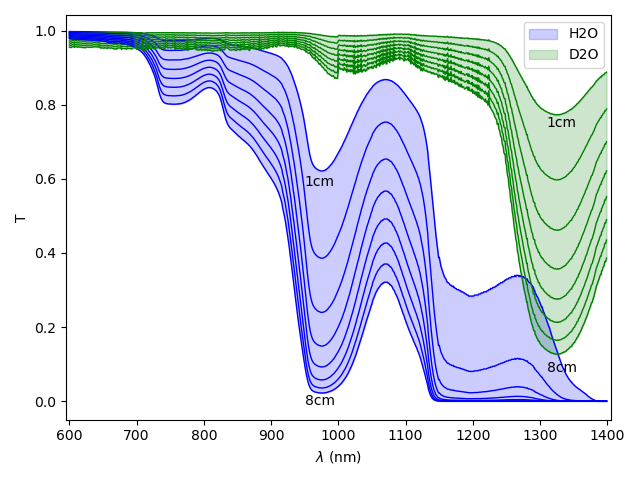
\includegraphics[width=0.7\textwidth]{./Figures/fiberfilling/water_transmission/water_transmission.png}
	\caption{The transmission of heavy water(green) and regular water(blue) is shown for slabs of thickness ranging from 1cm to 8cm in increments of 1cm using absorption data by \cite{kedenburg}. }
	\label{fig:water transmission}
\end{figure}
Fibers that are fully-filled with water will produce a frequency shift in the bandgap. On the other hand, when the core is selectively filled with water, the core refractive index will be greater than effective refractive index of the cladding and light will be guided via total-internal reflection. H${}_2$O, while widely available and a common solvent, has high absorption loss in the near infrared (NIR) but its most common isotope D${}_2$O has comparatively much less absorption loss in the same region (Fig.\ref{fig:water transmission}). The transmission in HCPCF are explored for H${}_2$O for its ubiquity while D${}_2$O for its suitability as a filling liquid in the NIR.
\clearpage
\subsection{Selective Filling}
\subsubsection{Filling Method}
To selectively fill the core of 800nm HCPCF, the photonic crystal cladding was collapsed while leaving the hollow-core open and is similarly filled with liquid using capillary action. The cladding is collapsed by placing the HCPCF opposite of a solid-core fiber in a fusion splicer \cite{xiao} and adjusting arc current duration and power to melt the cladding structure while remaining distanced enough to prevent fusion with the solid-core fiber.

\begin{figure}[!htb]
	\centering
	\foreach \x in {50ms 15mA, 70ms 20mA, 70ms 25mA, 80ms 25mA, 90ms 25mA, 100ms 25mA}
	{
		\begin{subfigure}[b]{0.3\textwidth}
			\includegraphics[width=\textwidth]{./Figures/fiberfilling/arc_power/\x.png}
			\caption{\x}
		\end{subfigure}
		\hfil
	}
	\caption{Side profile of collapsed cladding 1550HC fiber running the fiber splicer with varying current strength and duration. }
	\label{fig:selective filling}
\end{figure}
In Fig.\ref{fig:selective filling} the extent of collapse of the cladding is compared to various timing and power for an ORIENTEK T40 fusion splicer. The optimal setting is around an arc power of 25mA for a 70ms duration, though due to the imprecision in the arc power discharge the cladding on occasion will be overexposed, as shown in Fig.\ref{fig:selective err}.

\begin{figure}[!htb]
	\centering
	\foreach \x in {collapsed, fiberend}
	{
		\begin{subfigure}[b]{0.4\textwidth}
			\includegraphics[width=\textwidth]{./Figures/fiberfilling/arc_err/\x.jpg}
		\end{subfigure}
		\hfil
	}
	\caption{Variation between fibers using splicer settings 70ms 25ms  }
	\label{fig:selective err}
\end{figure}
\subsubsection{Transmission}
\begin{figure}[!htb]
	\centering
	\foreach \x in {HC800\_empty, HC800\_D2O, HC800\_H2O}
	{
		\begin{subfigure}[b]{0.32\textwidth}
			\includegraphics[width=\textwidth]{./Figures/fiberfilling/HC800/ModeShape/\x.png}
			\caption{}
		\end{subfigure}
		\hfil
	}
	\caption{Modeshape of 800 hollow-core fiber filled with (a)air (b)heavy water (c)DI water.}
	\label{fig:800 modeshape}
\end{figure}
\begin{figure}[!htb]
	\centering
	\includegraphics[width=0.75\textwidth]{./Figures/fiberfilling/HC800/transmission.png}
	\caption{Transmission of H${}_2$O and D${}_2$O in a selectively-filled 800nm hollow-core fiber.}
	\label{fig:trans 800hc}
\end{figure}
The air-filled 800nm HCPCF covers a transmission spectral range of 750nm–950nm. Light exits the fiber with a Gaussian mode shape, as shown in Fig.\ref{fig:800 modeshape}. In a H${}_2$O core, the coupling efficiency of the fiber drops to 31\%, while a heavy water filled core is less affected by absorption over this region and retains a coupling efficiency of up to 67\%.
\clearpage
\subsection{Full-Fiber Filling}
\subsubsection{Filling Method}
The air in 1550nm HCPCF was replaced with deionized water and heavy water by utilizing capillary action. 
\subsubsection{Transmission}
\begin{figure}[!htb]
	\centering
	\foreach \x in {HC1550_empty, HC1550_full_D2O, HC1550_H2O}
		{
			\begin{subfigure}[b]{0.32\textwidth}
				\includegraphics[width=\textwidth]{./Figures/fiberfilling/HC1550/ModeShape/\x.png}
				\caption{}
			\end{subfigure}
			\hfil
		}
	\caption{Modeshape of 1550 hollow-core fiber filled with (a)air (b)heavy water (c)DI water. Fiber filled with heavy water maintains a Gaussian profile while the fiber with regular distilled water shows some distortion.}
	\label{fig:1550 modeshape}
\end{figure}
The air-filled 1550nm HCPCF covers a transmission spectral range of 1200nm–1700nm. With a filled core and cladding, the spectral range shifts to transmitting wavelengths between 600nm–1100nm for both heavy water and water, confirming the scaling laws. Heavy water achieved a coupling efficiency of 47\%, but water only 16\%. While the D${}_2$O fiber modeshape retains a Gaussian profile, the H${}_2$O mode shape contains noise as some light also leaks from the photonic structure. The absorption effects of H${}_2$O severely reduce the transmission for wavelengths above 820nm, while compares well to the transmission of the D${}_2$O fiber below 820nm and could arguably be used as a filling liquid.
\begin{figure}[!htb]
	\centering
	\includegraphics[width=0.75\textwidth]{./Figures/fiberfilling/HC1550/transmission.png}
	\caption{Transmission of H${}_2$O and D${}_2$O in fully-filed and core-filled 1550nm hollow-core fiber.}
	\label{fig: trans 1550hc}
\end{figure}
\clearpage
